\section{Kjøretidsberegning}
\subsection{Om kjøretider}
For å vite hvor effektiv en algoritme er, ønsker man å vite hvor kjapp den er i forhold til hvor mye informasjon man sender inn. Noen ganger vil en dobling av antall inn-verdier bare øke kjøretiden med en konstant tid, andre ganger vil den doble kjøretiden, og ofte vil den øke med veldig mye.
\\\\
Kjøretider skal alltid oppgis med \textbf{asymptotisk notasjon}. Det vil si at man finner (teoretisk) matematisk funksjon for kjøretiden med antall inn-verdier som parameter. Deretter ser man på det leddet som dominerer mest i uttrykket når inn-verdiene blir store nok, og bruker dette (uten noe konstantledd) som et mål på hvor rask algoritmen er. Målet er at det ikke skal vokse særlig raskt.

\begin{boxed}
Anta at du har mange forskjellige tall, og du skal finne det største taller. Du sjekker da det første tallet, og setter denne som en midlertidig mulighet for at det er det største tallet. Deretter går du gjennom resten av tallene og sammenligner hver og en av dem med det tallet du antar er det største. Hvis du plukker opp et større tall enn du har fra før, setter du det nye til å være en mulighet for å være det største. Når du har gått gjennom alle tallene, vil det tallet du satte av som en mulig kandidat sist være det største tallet. Slik må det være, fordi da du plukket opp det største tallet satte du dette som en mulig kandidat og ingen andre tall var større. Dette gjelder selvsagt også om flere tall er like i verdi. Så lenge du ikke kunne ane hvor i bunken det største er da du begynte, vet du at du er nødt til å gå gjennom alle tallene en gang.
\newline \newline
På en andre siden trenger du ikke gå gjennom tallene flere ganger heller, for ved å bruke algoritmen beskrevet ovenfor, vet du at svaret er korrekt etter nøyaktig en gjennomgang (så lenge du ikke gjør noen feil underveis, vel og merke!). Hvis mengden med tall dobles og du antar at du alltid vil bruke like lang tid på hver sammenligning uansett hvor mange tall du har, vil arbeidstiden også dobles. Det kan f.eks. se slik ut:
\newline \newline
Du har tallene 2 3 1 7 5
\newline \newline
1. steg: Du sjekker tallet 2; 2 er nå kandidat til å være det største tallet.\\
2. steg: Du sjekker tallet 3; 3 er nå kandidat til å være det største tallet.\\
3. steg: Du sjekker tallet 1; 3 er fortsatt størst.\\
4. steg: Du sjekker tallet 7; 7 er nå kandidat til å være det største tallet.\\
5. steg: Du sjekker tallet 5; 7 er fortsatt størst.
\newline \newline
Nå som alle tallene er sjekket vet vi at 7 er det største tallet.
\end{boxed}

\noindent Kjøretider kan man finne ved å bruke iterasjon, rekursjonstre, variabelskifte, substitusjonsmetoden eller masterteoremet.

\subsection{$\theta$, $O$ og $\Omega$-notasjon}
Disse symbolene brukes for å sammenligne hvor fort forskjellige funksjoner vokser, og det er viktig at man blir kjent med bruken av dem. Noen ganger brukes $\theta$ og $O$-notasjonen om hverandre. Men hvis du har at en algoritme har en kjøretid på $O(n^2)$ mens den kanskje er $\theta(n)$ så er det jo riktig, selv om det jo er kjekt å vite at den er enda raskere enn det $\theta(n^2)$ er.
\\\\
I praksis brukes $\theta$-notasjon når det er et fast antall elementer du må undersøke hver gang. Det vil si at det er ikke snakk om å ha flaks eller uflaks med tallene. Noen ganger snakker vi om "worst case", "average case" og "best case" og bruker denne notasjonen i disse forskjellige tilfellene. Da må du ikke la deg lure til å tro at notasjonen gjelder kjøretiden til algoritmen generelt.
\\\\
$O$ brukes ofte om worst case og $\Omega$ om best case, men disse er ikke knyttet fast sammen. $O$, $\Omega$ og $\theta$ beskriver \textit{funksjoner}, uavhengig av hva det er disse funksjonene beskriver. Det er ikke noe i veien for f.eks. å si at worst case for en viss algoritme er $\Omega(n lg n)$, selv om dét sjelden er særlig nyttig. Det man ofte gjør, er følgende: sett at man har funnet ut at en algoritmes kjøretid er $\theta(n)$ i best case og $\theta(n^2)$ i worst case; da kan man si at kjøretiden generelt er $\Omega(n)$ og $\O(n^2)$.

\subsubsection{$\theta$-notasjon}
Denne notasjonen er den mest nøyaktige av de tre. Har du denne har du også de to andre. Her er $f(n)$ en funksjon som beskriver kjøretiden til en algoritme, hvor $n$ er størrelsen på inputen. $g(n)$ er et annet funksjonsuttrykk som vanligvis er enklere enn $f(n)$. Nå har vi at $\theta(g(n))$ defineres som følger:

\begin{center}
\textit{$\theta(g(n)) = \{ f(n)$: slik at det finnes positive konstanter $c_1$, $c_2$ og $n_0$ så vi har $0 \leq c_1 g(n) \leq f(n) \leq c_2 g(n)$ for alle $n_0 \leq n \}$}
\end{center}

\noindent Dette vil si at $f(n)$ blir skvist mellom to kurver som begge bare har en konstant forskjell, så lenge input-verdien $n$ er stor nok. Litt unøyaktig forklart betyr det at $f(n)$ vokser "omtrent like raskt som" $g(n)$.

\begin{boxed}
Anta at du vet at kjøretiden til en algoritme er gitt nøyaktig til å være $g(n) = \frac{1}{2}\ n^2 + 3n$. Da vil denne sies å ha kjøretid $\theta(n^2)$ fordi ved å velge $c_1$ mindre enn \(\frac{1}{2}\) og $c_2$ større enn \(\frac{1}{2}\) kan vi finne en eller annen stor nok $n$ slik at $c_1 n^2$ alltid er mindre enn \(\frac{1}{2}\)$n^2 + 3$ og $c_2 n^2$ alltid vil være større enn \(\frac{1}{2}\)$n^2 + 3$.
\end{boxed}

\begin{table}[H]
    \caption{Eksempler}
    \label{tab:kjoretideks}
    \centering
    \begin{tabular}{|L{5em} | L{35em}|}
        \hline
        \rowcolor[HTML]{303F9F}
        \textbf{\textcolor{white}{Kjøretid}} & \textbf{\textcolor{white}{Beskrivelse}}\\
        \rowcolor[HTML]{E6E6E6}
        $\theta(lg n)$ & Denne kalles logaritmisk kjøretid, og er fin-fin. Dette skjer blant annet hvis du kan halvere problemstørrelsen din ved å teste ett element. F.eks. kan du tenke deg at du vet at du har en \textbf{stigende tallfølge} og skal finne et bestemt tall. Da kan du sjekke det midterste. Hvis det er for lite, kan du se bort fra alle tallene i venstre halvdel, som du vet er mindre. Dermed har du allerede omtrent halvert problemstørrelsen din! Om tallet du ser på først er større, ser du bort fra alle tallene i høyre halvdel, som er større enn dette. Dersom tallet du leter etter eksisterer i tallfølgen, finner du det fort. Og hvorfor er kjøretiden $\theta(lg n)$? Jo, du starter med en rekkefølge med lengde $n$ som du halverer gang på gang helt til du er nede i lengde 1. Hvis antallet halveringer som trengs er $k$, har vi \(\frac{n}{2^k}\)$ = 1$. Løsningen av denne ligningen er $k = lg n$. Merk også at $lg 2n = lg 2 + lg n = 1 + lg n$ – en dobling av problemstørrelse gir kun et konstant tillegg til kjøretiden. \\
        $\theta(n)$ & Dette er en polynomisk kjøretid. Hvis du har en input på størrelse $n$, og er nødt til å gå gjennom alle tallene én gang, har vi enkelt og greit $\theta(n)$.\\
        \rowcolor[HTML]{E6E6E6}
        $\theta(n^2)$ & Nok et eksempel på en polynomisk kjøretid. Gitt at du har en input på $n$. Det forekommer ofte at man må lete gjennom en matrise som har $n$ rader og $n$ kolonner. I dette tilfellet vil en dobling av input gi fire ganger så mange elementer å lete gjennom!\\
        $\theta(2^n)$ & Her er vi inne på eksponentiell kjøretid. Denne er ikke morsom! Bare ett lite tillegg på input fra f.eks. en million til en million og én vil øke kjøretiden med det dobbelte. Dette kan forekomme ved at du for hvert element du tester, springer det ut to nye valg som du må teste.\\
         \hline
    \end{tabular}
\end{table}

\subsubsection{$O$-notasjon}
Til forskjell fra $\theta$-notasjonen vil $O$-notasjonen kun ta for seg den øvre begrensningen til funksjonen:

\begin{center}
\textit{$O(g(n)) = \{ f(n)$: slik at det finnes positive konstanter $c$ og $n_0$ så vi har $0 \leq f(n) \leq cg(n)$ for alle $n_0 \leq n \}$}
\end{center}

\noindent Dette er ikke så ulikt $\theta$-notasjonen. $2n^2 + 100n$ er både $\theta(n^2)$ og $O(n^2)$. Men den er også $O(n^3)$, $O(n^4)$, $O(2^n)$ og alt som verre er. For hvis en eller annen konstant ganget med $n^2$ alltid vil være større enn kjøretiden, så gjelder det også alle andre funksjoner som vokser raskere enn det igjen. Altså, hvis du vet at kjøretiden til den kan også være $\theta(n*log(n))$ eller $\theta(n)$ eller $\theta(log(n))$. Derimot kan den ikke være verre, f.eks. $\theta(n^3)$.

\subsubsection{$\Omega$-notasjon}
Der $O$-notasjonen ga en øvre begrensning for hvor raskt en fuksjon kan vokse, gir $\Omega$-notasjon en nedre begrensning. Derfor brukes ikke $\Omega$ så veldig ofte, for den vil aldri kunne gi en maksgrense for hvor lang tid en algoritme vil bruke, bare en minimumsgrense. Hvis du f.eks. viser at en algoritme har en kjøretid på $\Omega(n)$, så kan det godt hende at den egentlige kjøretiden er $2^n$, som er fryktelig dårlig. Det er omtrent som å si "jeg vil bruke minst ett minutt på å løse denne oppgaven" – da har du dine ord i behold hvis du bruker et helt år. Den formelle definisjonen av $\Omega$ er som følger:

\begin{center}
\textit{$\Omega(g(n)) = \{ f(n)$: slik at det finnes positive konstanter $c$ og $n_0$ så vi har $0 \leq cg(n) \leq f(n)$ for alle $n_0 \leq n \}$}
\end{center}

\noindent Kombinerer vi definisjonene av $O$ og $\Omega$ får vi definisjonen av $\theta$. Dette gjelder andre veien også: dersom du vet at $f(n) = O(g(n))$ og $f(n) = \Omega(g(n))$, vet du at $f(n) = \theta(g(n))$.

\subsection{Noen vanlige kjøretider}
Noen vanlige kjøretider er beskrevet i tabellen under. Sortert fra høyest til lavest.

\begin{table}[H]
    \caption{Kjøretider}
    \label{tab:kjoretider}
    \centering
    \begin{tabular}{|L{15em} | L{15em}|L{15em}|}
        \hline
        \rowcolor[HTML]{303F9F}
        \textbf{\textcolor{white}{Kompleksitet}} & \textbf{\textcolor{white}{Navn}} & \textbf{\textcolor{white}{Type}}\\
        \rowcolor[HTML]{E6E6E6}
        $\theta(n!)$ & Factorial & Generell\\
        $\Omega(k^n)$ & Eksponensiell & Generell\\
        \rowcolor[HTML]{E6E6E6}
        $O(n^k)$ & Polynomsik & Generell\\
        $\theta(n^3)$ & Kubisk & Tilfelle av polynomisk\\
        \rowcolor[HTML]{E6E6E6}
        $\theta(n^2)$ & Kvadratisk & Tilfelle av polynomisk\\
        $\theta(n log n)$ & Loglineær & Kombinasjon av lineær og logaritmisk\\
        \rowcolor[HTML]{E6E6E6}
        $\theta(n)$ & Lineær & Generell\\
        $\theta(lg n)$ & Logaritmisk & Generell\\
         \rowcolor[HTML]{E6E6E6}
        $\theta(1)$ & Konstant & Generell\\
         \hline
    \end{tabular}
\end{table}

\begin{table}[H]
    \caption{Kjøretider}
    \label{tab:kjoretider}
    \centering
    \begin{tabular}{|L{8em} | L{8em}|L{8em}| L{8em}|L{8em}|}
        \hline
        \rowcolor[HTML]{303F9F}
        \textbf{\textcolor{white}{Algoritme}} & \textbf{\textcolor{white}{Best-case}} & \textbf{\textcolor{white}{Average-case}} & \textbf{\textcolor{white}{Worst-case}} & \textbf{\textcolor{white}{Sammenligning}}\\
        \rowcolor[HTML]{E6E6E6}
        Bubblesort & $\theta(n)$ & $\theta(n^2)$ & $\theta(n^2)$ & Ja\\
        Insertion sort & $\theta(n)$ & $\theta(n^2)$ & $\theta(n^2)$ & Ja\\
        \rowcolor[HTML]{E6E6E6}
        Selection sort & $\theta(n^2)$ & $\theta(n^2)$ & $\theta(n^2)$ & Ja\\
        Heapsort & $O(n lg n)$ & $O(n lg n)$ & $O(n lg n)$ & Ja\\
        \rowcolor[HTML]{E6E6E6}
        Quicksort & $\theta(n lg n)$ & $\theta(n lg n)$ & $\theta(n^2)$ & Ja\\
        Merge sort & $\theta(n lg n)$ & $\theta(n lg n)$ & $\theta(n lg n)$ & Ja\\
        \rowcolor[HTML]{E6E6E6}
        Counting sort & $\theta(n + k)$ & $\theta(n + k)$ & $\theta(n + k)$ & Nei\\
         \hline
    \end{tabular}
\end{table}

\subsection{Kjøretiden til rekurrensligninger}
En rekurrensligning er en ligning som beskriver en funksjon ved dens verdi for mindre inn-verdier. 

\begin{boxed}
Fibonacci-tallene kan defineres som:
\begin{center}
$f(0) = f(1) = 1$\\
$f(n) = f(n-1) + f(n-2)$
\end{center}
\noindent For å finne det $n$-te Fibonacci-tallet må man altså kjenne de to foregående tallene. De fem første tallene blir 1 1 2 3 5.
\end{boxed}

\noindent Selv om Fibonacci-tallene kan løses som rekurrensligning, vil dette bli en eksponentiell kjøretid. Heldigvis finnes det langt smartere måter å løse denne på enn ved rekursjon.
\\\\
Det er i hovedsak tre metoder som brukes for å finne kjøretiden til rekurrensligninger; substitusjonsmetoden, rekurrenstre, og mastermetoden.

\subsubsection{Substitusjonsmetoden}
Denne metoden løser rekurrensligninger gjennom to steg:
\begin{enumerate}
    \item Gjett på en løsning
    \item Bruk \textbf{matematisk induksjon} til å verifisere eller forkaste den mulige løsningen.
\end{enumerate}

\noindent Det kan virke vanskelig å gjette på riktig løsning, men dette er faktisk ikke så veldig stort problem. Med litt trening ser man sånn omtrent hvor den vil ligge hen. Og mulighetene er egentlig ikke så veldig mange. Det blir som regel $\theta$ av $n$, $n^2$ eller $n^3$, eventuelt multiplisert med $log(n)$.

\begin{boxed}
Anta at rekurrensen er beskrevet ved:
\begin{center}
$T(n) = 2T(\lfloor n/2 \rfloor)+\(\frac{1}{2}\)n$  $\lfloor$ ... $\rfloor$ betyr å runde ned til nærmeste heltall
\end{center}
\noindent Vi kan da gjette på at løsningen er $O(n * log(n))$. Det vi da må vise, er at $T(n) \leq c * n * log(n)$ for en eller annen konstant $c > 0$. Ved å sette inn dette forslaget, vil man finne ut at for $c \geq 1$ fungerer det. Hadde vi mislykkes, måtte vi ha prøvd med en dårligere kjøretid. Og dessuten må man finne ut om det ikke finnes enda bedre kjøretider. 
\end{boxed}

\subsubsection{Rekurrenstre}
Om du fortsatt ikke liker tanken på å gjette i vildens sky kommer rekurrenstremetoden som kallet. I rekurrenstreet vil hver node representere kostnaden av et enkelt underproblem. Vi summerer kostnadene på hvert nivå av treet for å finne kostnaden per nivå, og deretter summerer vi alle kostnadene per nivå for å finne total kostnad til alle nivåene. Dette høres kanskje komplisert ut med er ganske greit. Lager man treet svært nøye, kan det holde som et bevis i seg selv. Eller man kan finne noen tall og se hva slags \textbf{asymptotisk oppførsel} de har, for deretter å verifisere gjettingen ved substitusjonsmetoden.

\begin{boxed}
Rekurrenstreet til $T(n) = 3T(n/2) + cn^3$ er vist i figur \ref{fig:rekurrenstre} under. Vi ser at arbeidet i første nivå er $cn^3$, det samlede arbeidet i andre nivå er $3c$\(\frac{n^3}{2}\) osv. Vi regner med at rekursjonen stopper når argumentet til funksjonen er blitt 1. Siden argumentet starter på $n$ og halveres i hvert nivå, vil treet he $lg n$ nivåer. Samlet kjøretid blir da $\Sigma_{1=0}^{lg n} 3^i (\frac{n}{2^i}\))^3$.

\begin{figure}[H]
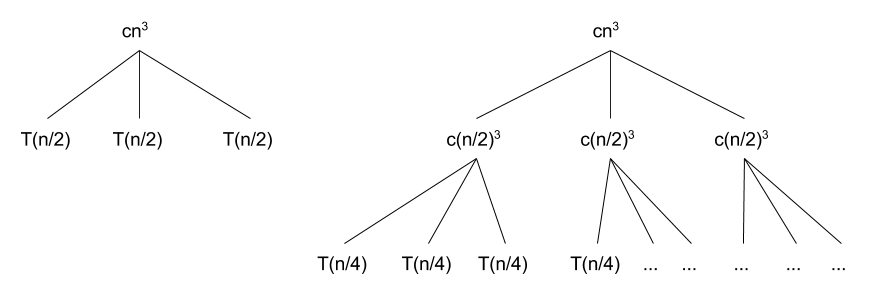
\includegraphics[scale=0.5]{images/rekurrenstre}
\centering %centering the image
\caption{Rekurrenstre}
\label{fig:rekurrenstre}
\end{figure}

\noindent Se Cormen side 64.
\end{boxed}

\subsubsection{Master-metoden}
Selve kokebokmetoden. Hvis du har en rekurrensligning på formen:
\begin{center}
$T(n) = aT(n/b) + f(n)$
\end{center}
\noindent Hvor $a \geq 1$ og $b > 1$ er konstanter og $f(n)$ er en asymptotisk, positiv funksjon, så er det bare å bruke masterteoremt rett fram. Se side 73 i Cormen. I korte trekk sier den at om du lar $n/b$ bety enten $\lfloor n/b \rfloor$ eller $\lceil n/b \rceil$ så har du:

\begin{enumerate}
    \item Hvis $f(n) = O(n^{log_b a-\epsilon})$ for en konstant $\epsilon > 0$, \Rightarrow $T(n) = \theta(n^{log_b a})$
    \item Hvis $f(n) = \theta(n^{log_b a})$, \Rightarrow $T(n) = \theta(n^{log_b a} * log(n))$
    \item Hvis $f(n) = \Omega(n^{log_b a+\epsilon})$ og hvis $a f (n/b) \leq c f (n)$ for en konstant $c > 1$ og $n$ stor nok, \Rightarrow $T(n) = \theta(f(n))$
\end{enumerate}

\begin{boxed}
Anta at du har:
\begin{center}
$T(n) = 9T(n/3) + n$
\end{center}
\noindent Her er $a = 9$, $b = 3$ og $f(n) = n$. Vi ser at:
\begin{center}
$n^{log_3 9} = n^2 = \theta(n^2)$
\end{center}
\noindent Siden $f(n) = O(n^{log_3 9-\epsilon}$ med $\epsilon = 1$, så gir første del av masterteoremet at $T(n) = \theta(n^2)$.
\end{boxed}
